\documentclass[10,a4paperpaper,]{article}

  \title{Reporte interactivo sobre funcionarios públicos}
  \author{Jorge Hernández, Eugenio Mora}
  \date{\today}
  


\newcommand{\logo}{logo.png}
\newcommand{\cover}{cover.png}
\newcommand{\iblue}{2b4894}
\newcommand{\igray}{d4dbde}

% Author: Karol KozioL
% License: GPL-3
% Modified by: Sarah Wagner

% % % packages -----------------------------------------------------------------------------------
\usepackage{amsmath}
\usepackage{array}
\usepackage{booktabs}
\usepackage{calc}
\usepackage{eso-pic}
\usepackage{fancyhdr}
\usepackage{fontspec}
\usepackage[left = 2.5cm, right = 2.5cm, top = 1.2cm, bottom = 1.2cm, includeheadfoot]{geometry}
\usepackage{graphicx}
\usepackage[utf8]{inputenc}
\usepackage{lastpage}
\usepackage{multirow}
\usepackage{tabularx} 
\usepackage{tikz}
\usepackage{titlesec}
\usepackage{xcolor, colortbl}

% % % settings -----------------------------------------------------------------------------------

% % custom colors
\definecolor{iblue}{HTML}{\iblue}
\definecolor{igray}{HTML}{\igray}

% definition of pagename
\newcommand\pagename{Page}

% % fonts 
\defaultfontfeatures{Mapping = tex-text}
\setmainfont[BoldFont = Lato-Bold.ttf, ItalicFont = Lato-Italic.ttf, BoldItalicFont = Lato-BoldItalic.ttf]{Lato-Regular.ttf}
\newfontfamily\headingfont[ItalicFont = Lato-BlackItalic.ttf]{Lato-Black.ttf}


% % sections
\titleformat{\section}{\color{iblue}\headingfont\Large\bfseries}{\thesection}{1em}{}[\titlerule]
\titleformat{\subsection}{\color{iblue}\headingfont\large\bfseries}{\thesubsection}{1em}{}
\titleformat{\subsubsection}{\color{iblue}\headingfont\bfseries}{\thesubsubsection}{1em}{}

% % misc
\setlength{\parindent}{0em} 
\linespread{1}
\raggedright
\newcolumntype{C}{>{\centering\arraybackslash}X}


% % % custom titlepage ----------------------------------------------------------------------------
\newcommand\BackgroundPic{%
	\put(0,0){%
		\parbox[b][\paperheight]{\paperwidth}{%
			\vfill
			\centering
			
\includegraphics[width=\paperwidth,height=\paperheight]{\cover}%
			\vfill
}}}

\makeatletter

% pagestyle titlepage
\fancypagestyle{customtitle}{
	\lhead{}
	\chead{}
	\rhead{}
	\makeatother
	\lfoot{}
	\cfoot{}
	\rfoot{
\includegraphics{\logo}}
}


% titlepage
\renewcommand{\maketitle}{
	\thispagestyle{customtitle}
	\AddToShipoutPicture*{\BackgroundPic}
	\ClearShipoutPicture
	
	\phantom{a}\hfill
	\vspace{14cm}
	
	\begin{tabular}[l]{@{}p{\textwidth}@{}}
		\color{iblue}\headingfont\LARGE\@title\\[1em]
		\color{iblue}\headingfont\large\@author\\[1em]
		\color{iblue}\headingfont\small\@date\\[1em]
	\end{tabular}
	
	
	
	\clearpage
}
\makeatother

% % % header and footer ---------------------------------------------------------------------------
\pagestyle{fancy}
\lhead{}
\chead{}
\rhead{ 
\includegraphics{\logo}}
\makeatother
\newlength{\myheight}
\lfoot{}
\cfoot{}
\rfoot{\pagename~\thepage \hspace{1pt} / \pageref{LastPage}}
\renewcommand\headrulewidth{0pt}
\renewcommand\footrulewidth{0pt}




\begin{document}


\renewcommand{\contentsname}{Tabla de contenidos}

\renewcommand{\pagename}{Página}


\maketitle
\tableofcontents
\addcontentsline{toc}{section}{Contenido}
\clearpage

\section{Introducción}

Este reporte tiene como objetivo el recopilar y clarificar la
información que ya se encuentra filtrada dentro de la aplicación web.
Sabemos que tener un dashboard con la información actualizada al momento
es algo bastante útil, sin embargo, puede que no en todo momento
tengamos la oportunidad o facilidad de poder acceder a este, sobre todo
si nos encontramos en un entorno de actualización de datos en la nube,
por lo que con este reporte podrás descargar de manera interactiva los
datos ya filtrados en el dashboard.

\section{Sobre los hallazgos encontrados}

Dentro de las bases de datos, nos vamos a enfocar principalmente en la
primera y la tercera, considerando como métricas principales los
ingresos de los funcionarios públicos y los casos en los que existe un
conflicto de interés. Si bien es cierto que los ingresos pueden variar
dependiendo de los puestos, años de experiencia y otras variables
externas, vamos a considerar aquellos ingresos que sean sumamente altos
respecto a la media ponderada de los datos, haciendo uso de un
\texttt{boxplot} para encontrar aquellos datos que se encuentren fuera
de un cierto rango normal. Ahora, los ingresos promedio pueden variar de
estado a estado, como se puede ver en el gráfico siguiente, por lo que
vamos a seccionar los datos por estado para evitar un sesgo en esta
métrica.

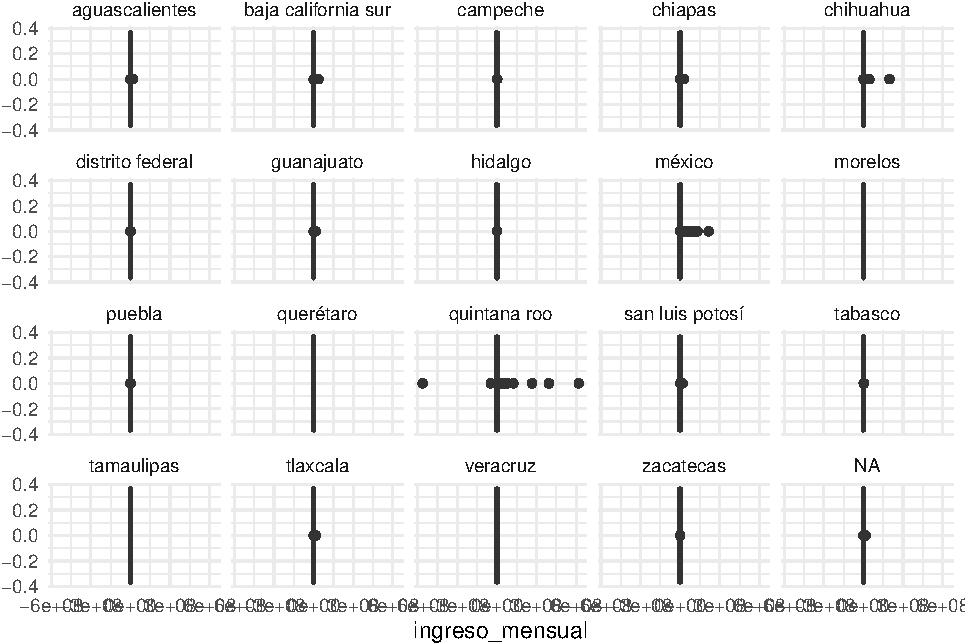
\includegraphics{report_files/figure-latex/unnamed-chunk-2-1.pdf}

Como segundo punto importante a considerar es si el usuario tiene un
conflicto de interés, lo cual lo vuelve un candidato potencial a
presentar algún caso de corrupción en un futuro. Para dar una
calificación de riesgo a los funcionarios, se hará uso de la siguiente
fórmula:

\[
Calificación = (\frac{I_e}{max (I_e)}+C_i)*100
\] La lógica de la fórmula es sencilla: Vamos a considerar una
ponderación respecto a los ingresos reportados que vaya de 0 a 1 (o
números negativos en caso de tener un ingreso negativo reportado),
siendo que la calificación máxima posible de obtener en este aspecto
será para la persona que haya reportado el mayor ingreso, mientras que
los casos de conflicto de interés se van a considerar como un punto.
Para una mejor comprensión de los datos visualmente, estos se van a
multiplicar por 100, de tal manera que la calificación de máximo riesgo
será de 200. Cabe aclarar que estos datos solo aplicarán para aquellos
casos en los que se considere que haya ingresos por encima de la media
ponderada.

Pasemos a ver un top con la información seleccionada en el reporte
anterior:

\begin{tabular}{l|l|l|r|l|r|r|r}
\hline
Nombre & Apellido & Seg apellido & C. de interés & Estado & Ingreso & P. por ingreso & Calificación\\
\hline
Freddy & Espinosa & Ramirez & 0 & NA & 15760672 & 1.000 & 100.000\\
\hline
Maria luisa & Villarreal & Novelo & 0 & NA & 4762732 & 0.302 & 30.219\\
\hline
Doris lucia & Pech & Chable & 0 & NA & 3934932 & 0.250 & 24.967\\
\hline
Maria del carmen & Suarez & Chan & 0 & NA & 3602326 & 0.229 & 22.856\\
\hline
Luis fernando & Peraza & Tun & 0 & NA & 3591066 & 0.228 & 22.785\\
\hline
Guillermo & Rodriguez & Alvarez & 0 & NA & 3230505 & 0.205 & 20.497\\
\hline
Gladys beatriz & Caballero & Centurion & 0 & NA & 3046594 & 0.193 & 19.330\\
\hline
Cristina beatriz & Bracamonte & Noh & 0 & NA & 2808835 & 0.178 & 17.822\\
\hline
Teresita de jesus & Caballero & Centurion & 0 & NA & 2666690 & 0.169 & 16.920\\
\hline
Selene alicia & Yah & Vargas & 0 & NA & 2556477 & 0.162 & 16.221\\
\hline
\end{tabular}

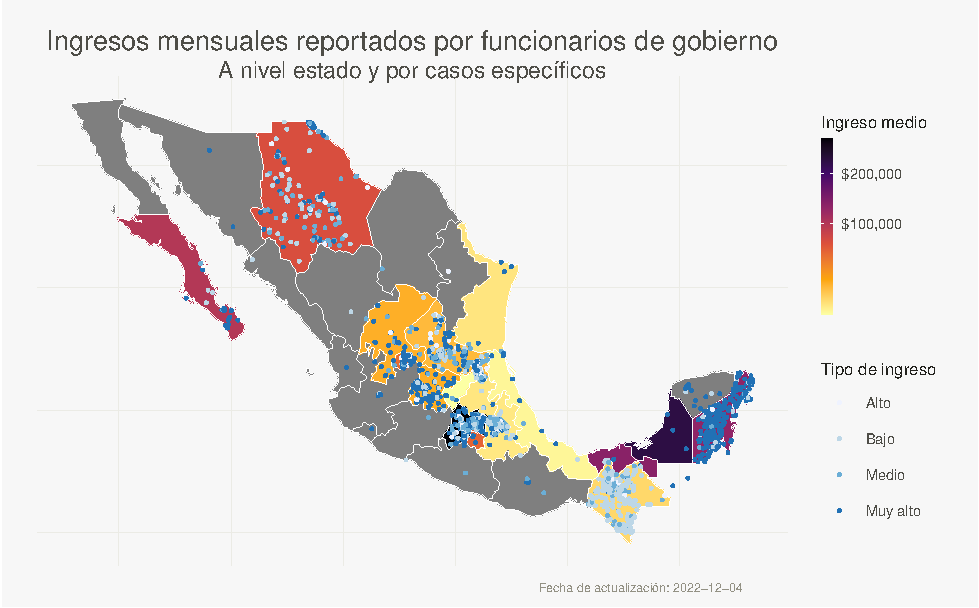
\includegraphics{report_files/figure-latex/unnamed-chunk-4-1.pdf}

\subsection{First Subsection}

At vero eos et accusamus et iusto odio dignissimos ducimus qui
blanditiis praesentium voluptatum deleniti atque corrupti quos dolores
et quas molestias excepturi sint occaecati cupiditate non provident,
similique sunt in culpa qui officia deserunt mollitia animi, id est
laborum et dolorum fuga. Et harum quidem rerum facilis est et expedita
distinctio.


\end{document}
